Понятие функции источника и формула \eqref{equ:equSourceFunction3} имеют место и для неограниченного пространства, если рассматривать функции, регулярные на бесконечности. Найдём функцию источника для полупространства $z > 0$. Поместим в точку $A(x_0, y_0, z_0)$ единичный заряд, который создаёт в неограниченном пространстве поле, потенциал которого определяется функцией
\begin{equation}
	\frac{1}{4 \pi} \frac{1}{R_{AM}}, \quad \mbox{где} \quad R_{AM} = \sqrt{(x - x_0)^2 + (y - y_0)^2 + (z - z_0)^2}
	\label{equ:equSourceFunHalfSpat}
\end{equation}

\begin{figure}[h!]
	\centering	
	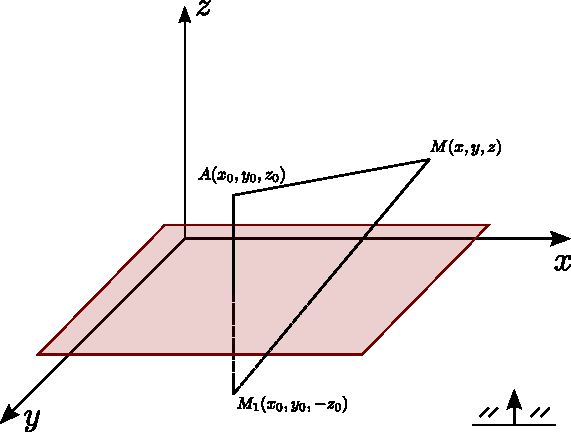
\includegraphics[scale=1]{figHalfSpatial.pdf}
\end{figure}
Нетрудно видеть, что <<индуцированное поле>> $v$  является полем отрицательного единичного заряда, помещённого в точку $M_1 (x_0, y_0, - z_0)$, являющуюся зеркальным изображением точки $M_0$ в плоскости $z = 0$. Функция $G$, равная 
\[
	G(M, A) = \frac{1}{4 \pi R_0} - \frac{1}{4 \pi R_1}
\]
где 
\begin{align}
	R_0 = \abs{\overrightarrow{AM}} &= \sqrt{(x - x_0)^2 + (y - y_0)^2 + (z - z_0)^2}\\
	R_1 = \abs{\overrightarrow{M_1M}} &= \sqrt{(x - x_0)^2 + (y - y_0)^2 + (z + z_0)^2}
\end{align}
обращается в нуль при $z = 0$ и имеет ненужную особенность в точке $A$.

Вычислим $\left. \derp{G}{n}{}\right|_{z = 0} = - \left. \derp{G}{z}{}\right|_{z = 0}$. Очевидно, что
\[
	\derp{G}{z}{} = \frac{1}{4 \pi} \left[ - \frac{z - z_0}{R_0^3} + \frac{z + z_0}{R_1^3} \right].
\]
Полагая $z = 0$, находим:
\[
	\left. \derp{G}{n}{} \right|_{z = 0} = \left. - \frac{G}{z}\right|_{z = 0} = - \frac{z_0}{2 \pi R_0^3}.
\]
Решение первой краевой задачи даётся формулой 
\[	
	u(A) = \frac{1}{2 \pi} \iint\limits_S \frac{z_0}{R_{AP} }f(p)\, d\sigma_P
\]
где $S$ -- плоскость $z = 0$, $f(P) = u|_{z = 0}$, или
\[
	u(x_0, y_0, z_0) = \frac{1}{2 \pi} \int\limits_{-\infty}^{\infty} \int\limits_{- \infty}^{\infty} \frac{z_0}{\left[(x - x_0)^2 + (y - y_0)^2 + z_0^2 \right]^{\frac{3}{2}}} f(x, y)\, dx dy
\]
%Для данной задачи мы должны построить функцию Грина.
%\[
%	G = W - \frac{1}{r_{AP}} = \frac{B}{r_{AP} - \frac{1}{r_{AP}}}
%\]
%\[
%	G|_{z = 0} = \left(\frac{B}{r_{AP} - \frac{1}{r_{AP}}} \right)_{z = 0} = 0
%\]
%\[
%	r_{AP} = \sqrt{(x - x_0)^2 + (y - y_0)^2 + (z - z_0)^2}
%\]
%\[
%	r_{A*P} = \sqrt{(x - x_0)^2 + (y - y_0)^2 + (z + z_0)^2}
%\]
%\[
%	z = 0 \to r_{AP} = r_{A*P}
%\]
%Нормаль направлена в сторону противоположную $z$, следовательно $\derp{G}{n}{} = - \derp{G}{z}{}$
%\[
%	G = \frac{1}{r_{AP}} - \frac{1}{r_{AP}}; - \derp{G}{z}{} = \frac{1}{r_{A*P}^2} \derp{r_{A*P}}{z}{} - \frac{1}{r_{AP}^2} \derp{r_{AP}}{z}{} = \frac{(z + z_0)}{r_{A*P}^3} - \frac{(z - z_0)}{r_{AP}^3} |_{z = 0} = \frac{2 z_0}{r_{AP}^3}
%\]
%Перейдём к формуле Грина \eqref{equ:equMainGreen3d}
	
%\begin{multline*}
%	4 \pi u(x_0, y_0, z_0) = \iint\limits_{S} u \derp{G}{n}{} dS = - \int\limits_{- \infty}^{+ \infty} dx \int\limits_{- \infty}^{+ \infty} dy f(x, y) \derp{G}{z}{} = \\ = - 2 z_0 \int\limits_{- \infty}^{+ \infty} dx \int\limits_{- \infty}^{+ \infty} \frac{f(x,y)}{\left[(x - x_0)^2 + (y - y_0)^2 +z_0^2 \right]^\frac{3}{2}} dy = \\ = [(x - x_0)^2 + (y - y_0)^2 +z_0^2 = x^2 + y^2 + x_0^2 + y_0^2 + z_0^2 - 2x x_0 - 2 y y_0] = \\ = \rho^2 + \rho_0^2 - 2 \rho \rho_0 \cos \theta \cos \theta_0 - 2 \rho \rho_0 \sin \theta \sin \theta_0] = \\ = - 2 z_0 \int\limits_{0}^{2 \pi} d\theta \int\limits_{0}^{\infty} \frac{f(\rho, \theta) \rho d\rho}{[\rho^2 + \rho_0^2 - 2 \rho \rho_0 \cos \theta \cos \theta_0 - 2 \rho \rho_0 \sin \theta \sin \theta_0]^\frac{3}{2}}
%\end{multline*}
%	$\iint\limits_S \left( u \derp{G}{n}{} - G \derp{u}{n}{}\right)dS + \iiint\limits_{\omega} = \begin{cases}
%		4 \pi &\mbox{если точка}\, A\, \mbox{лежит внутри}\, W\\
%		2 \pi &\mbox{если точка}\, A\, \mbox{лежит на границе}\, S\\
%		0 & \mbox{если точка}\, A\, \mbox{лежит вне}\, W
%	\end{cases}$\\

%Для пространственной задачи фундаментальным решением является $	\frac{1}{r}$ \\
%В плоском случае фундаментальным решением является 
%\[
%	\ln \frac{1}{r}
%\]
%\[
%	\Delta u = 0 \quad \derp{u}{x}{2} + \derp{u}{y}{2} = 0
%\]
%\[
%	r = \sqrt{(x - x_0)^2 + (y - y_0)^2}
%\]
%\[
%	u = \ln \frac{1}{r} = - \ln r
%\]
%Найдём производную\\
%\[
%	\derp{u}{x}{} = - \frac{1}{r} \derp{r}{x}{} = - \frac{1}{r^2}
%\]
%\[
%	\derp{u}{x}{2} = - \frac{1}{r^2} + \frac{2 (x - x_0)^2}{r^4}
%\]
%\[
%	\derp{u}{yx}{2} = - \frac{1}{r^2} + \frac{2 (y - y_0)^2}{r^4}
%\]
%\[
%	\derp{u}{x}{2} = \derp{u}{y}{2} = - \frac{2}{r^2} + \frac{2 [(x - x_0)^2 + (y - y_0)^2]}{r^4} = - \frac{2}{r^2} + \frac{2}{r^2} = 0
%\]

%Функцию Грина будем строить в  виде:\\
%\[
%	G = W - \ln \frac{1}{r_{AP}}
%\]
%В случае, если решаем задачу Дирихле, то для функции $G$:
%\[
%	\Delta G = 0
%\]
%\[
%	G|_S = 0
%\]

%Формула (2) будет иметь вид:\\
%\[
%	\oint\limits_{GR} \left(u \derp{v}{n}{} - v \derp{u}{n}{}\right) d \gamma = \iint\limits_S \left(u \Delta v - v \Delta u \right) dS
%\]
%\[
%	\oint\limits_{GR} \left(u \derp{v}{n}{} - v \derp{u}{n}{}\right) d \gamma + \oint\limits_{GR_1} \left(u \derp{v}{n_1}{} - v \derp{u}{n_1}{}\right) d \gamma = 0
%\]

%\begin{figure}[h!]
%	\centering	
%	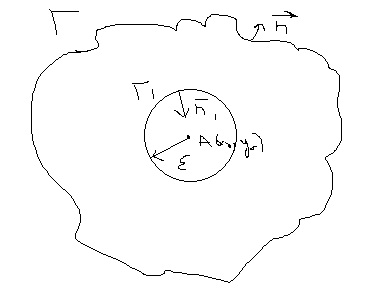
\includegraphics{8.jpg}
%\end{figure}
%Если интеграл берётся по окружности $\varepsilon$, то $\derp{}{n_1}{} = - \derp{}{r}{} \quad d \gamma = \varepsilon d \theta$
%\[
%	\oint\limits_{GR_1} \left(u \derp{v}{n_1}{} - G \derp{u}{n_1}{}\right) d \gamma = \int\limits_{0}^{2 \pi} \left(-u \derp{v}{r}{} - G \derp{u}{r}{}\right) \varepsilon d \theta = \int\limits_{0}^{2 \pi} \left(- u \derp{W}{r}{} + W \derp{u}{r}{} + u \derp{}{r}{} (\ln \frac{1}{r}) - \ln \frac{1}{r} \derp{u}{r}{}\right) \varepsilon d \theta
%\]
%\[
%	(- \ln r)' = - \frac{1}{r}
%\]
%Перейдём к пределу\\
%\[
%	\lim\limits_{\varepsilon \to 0} \varepsilon  \int\limits_{0}^{2 \pi} \left(-u \derp{W}{r}{} + W \derp{W}{r}{} \right) d \theta - \lim\limits_{\varepsilon \to 0} \varepsilon \int\limits_{0}^{2 \pi} [u \frac{1}{\varepsilon} + \derp{u}{r}{} \ln \varepsilon] d \theta
%\]
%Непрерывные фукнции
%так как интегрируем по очень маленькой области u можно заменить u с точкой.
